\documentclass[12pt, letterpaper]{report}
\usepackage[utf8]{inputenc}
\usepackage{newunicodechar}
\usepackage{pdfpages}
\usepackage{graphicx}
\usepackage{listings}
\usepackage{caption}
\usepackage{graphicx}
\usepackage{hyperref}
\usepackage{amsmath}

\title{ECE457B Assignment 4}
\author{David YeounJun Park \\ Student ID: 20434264}

\lstdefinestyle{mystyle}{
    backgroundcolor=\color{black},   
    commentstyle=\color{codegreen},
    keywordstyle=\color{magenta},
    numberstyle=\tiny\color{codegray},
    stringstyle=\color{codepurple},
    basicstyle=\footnotesize,
    breakatwhitespace=false,         
    breaklines=true,
    postbreak=\raisebox{0ex}[0ex][0ex],
    {\ensuremath{\color{red}\hookrightarrow\space}},                 
    captionpos=b,                    
    keepspaces=true,                 
    numbers=left,                    
    numbersep=5pt,                  
    showspaces=false,                
    showstringspaces=false,
    frame=single
}

\lstset{
    frame=single,
    breaklines=true,
    postbreak=\raisebox{0ex}[0ex][0ex]{\ensuremath{\color{red}\hookrightarrow\space}}
}

\begin{document}

\begin{titlepage}
\maketitle
\end{titlepage}

\section*{Problem 1}
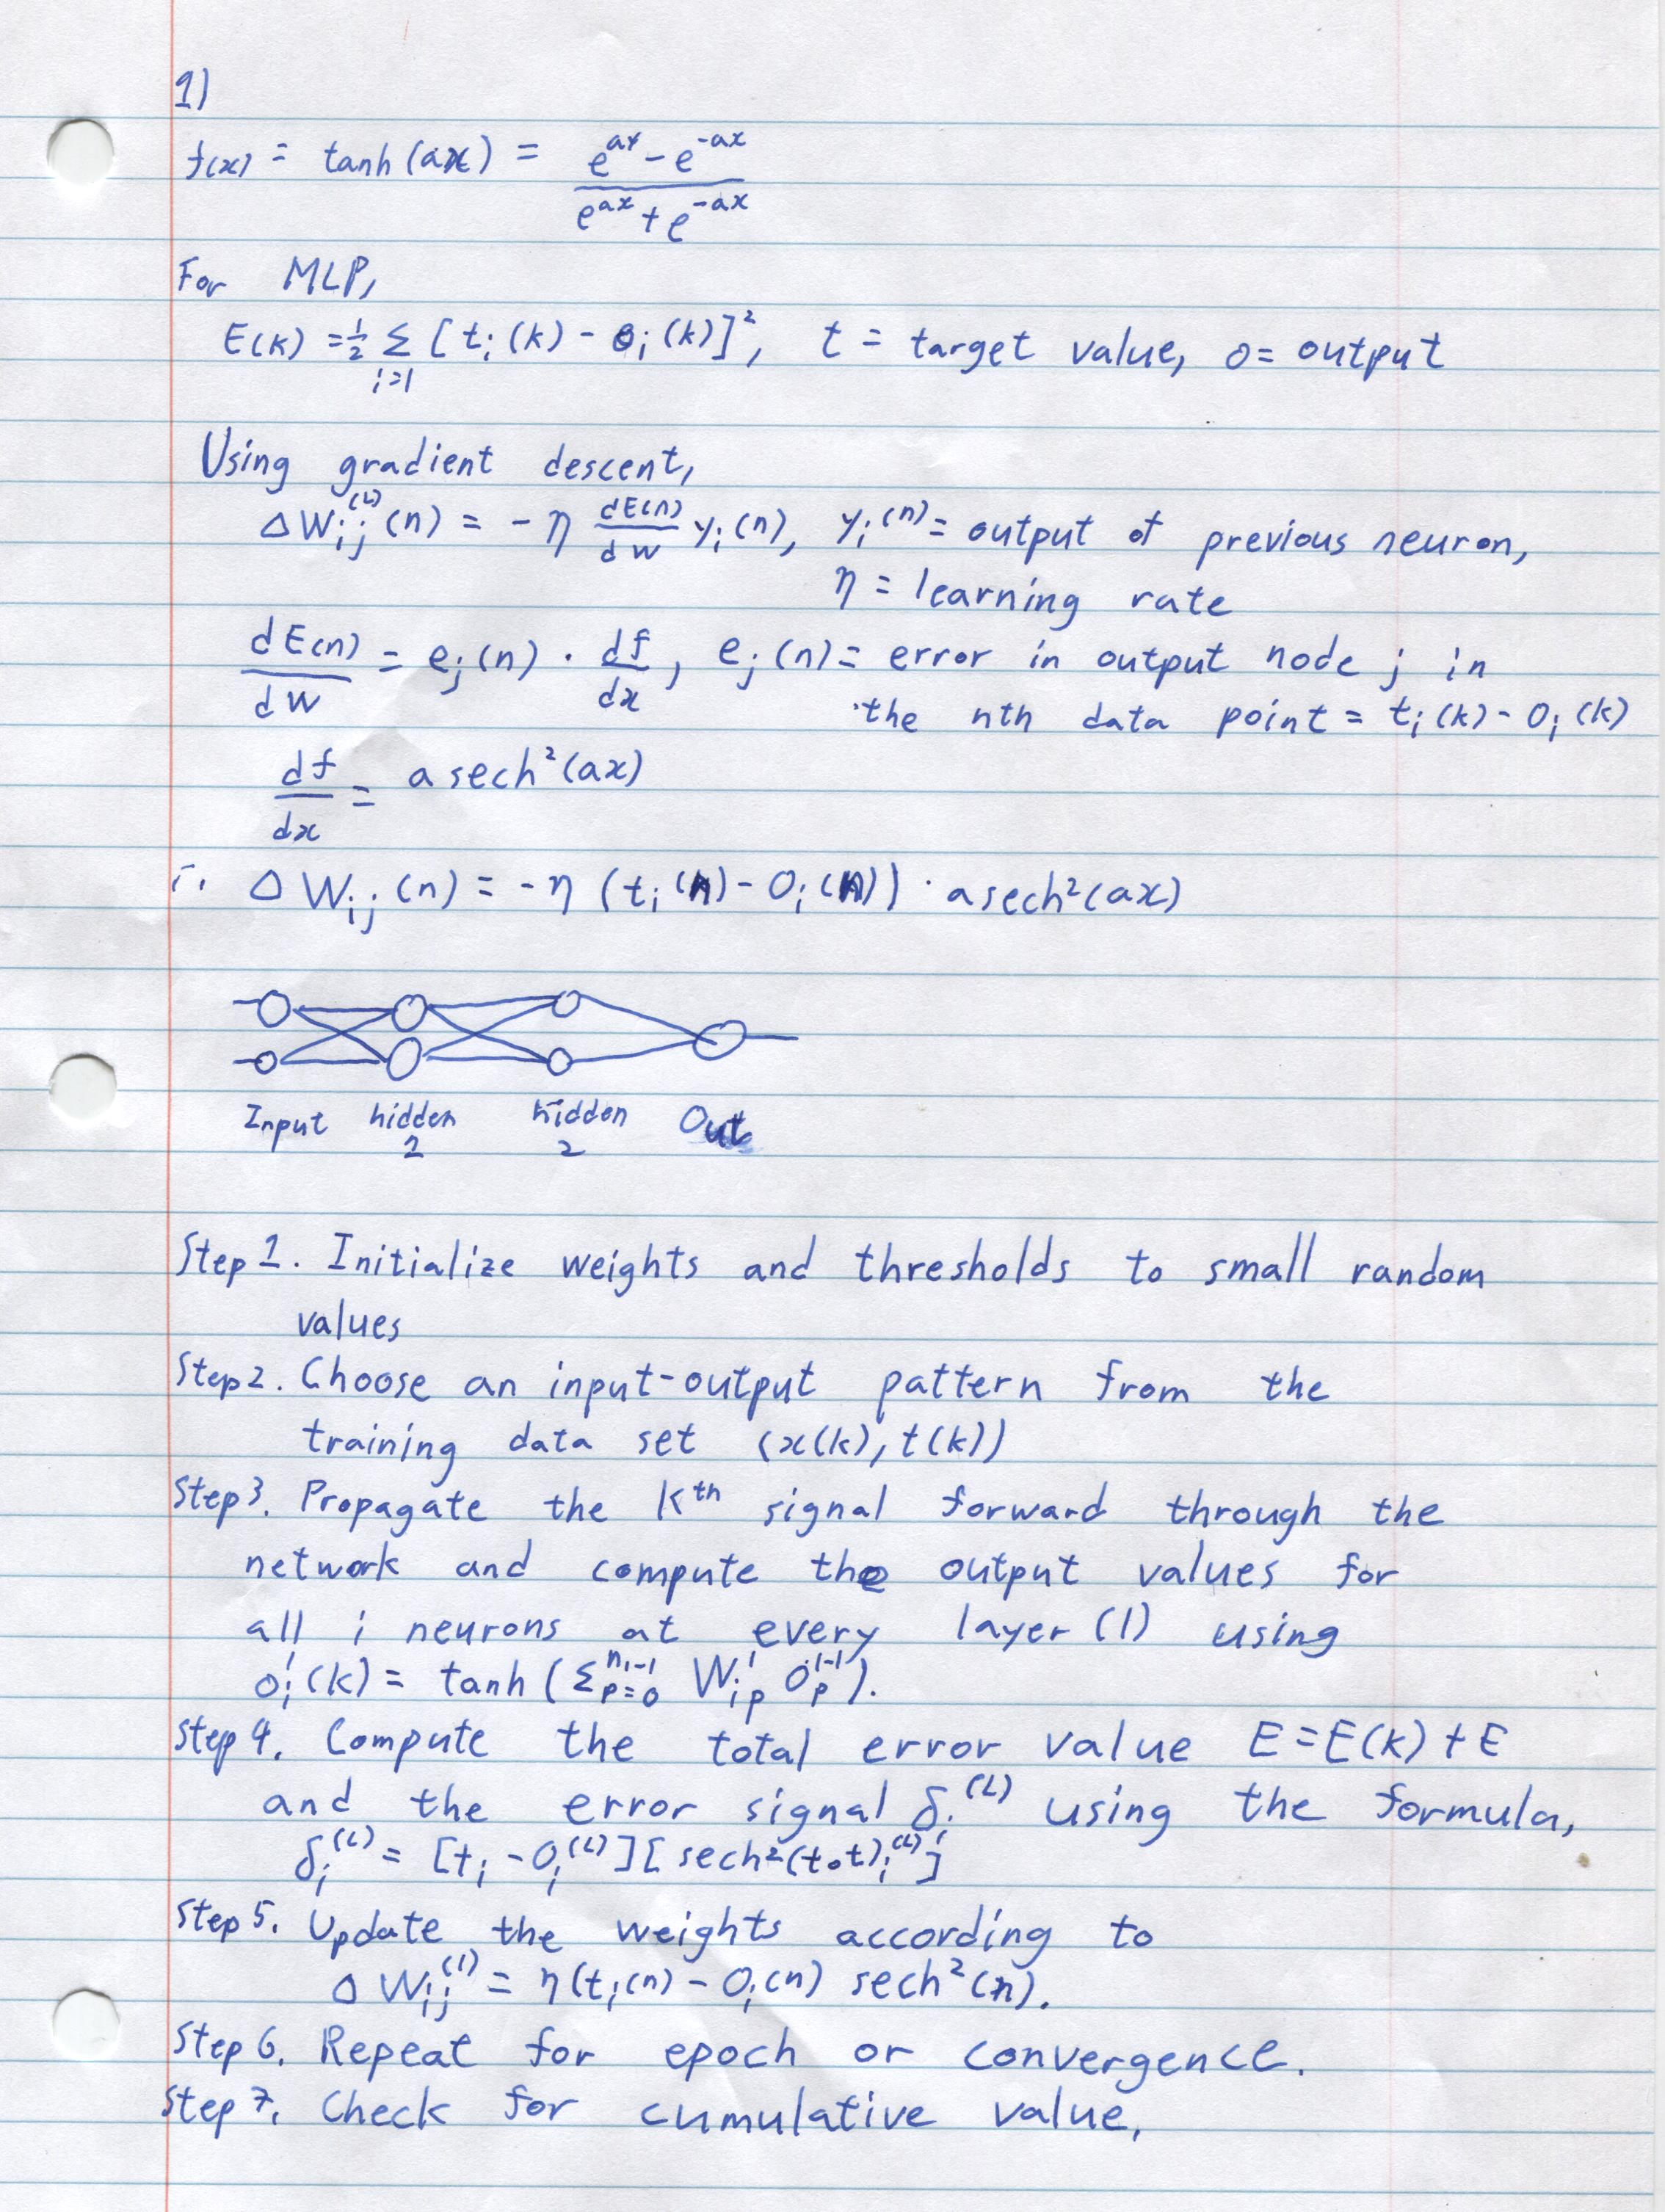
\includegraphics[scale=0.8]{001.jpg}
\section*{Problem 2}
\[f_a(x) = exp(-x^2)\]
\[f_b(x) = arctan(x)\]
\subsection*{Section A}
\paragraph*{} The network uses sigmoid function. It has 1 input, 1 hidden layer with 3 nodes, and 1 output layer. The learning rate is 0.1, with 0 momentum.
\paragraph*{} The number of hidden nodes are fixed to 3 nodes. First, 5 points were generated with the even distribution for the range of each function for training. Then, 5 more points were generated with the even distribution for the range of each function for validation. Then the network was trained until convergence. The total errors were
\[Error_{tot}(f_a(x)) = 0.822\]
\[Error_{tot}(f_b(x)) = 0.0669\]
\paragraph*{} Then, 10 points were generated with the even distribution for the range of each function for the training. The validation list remained same. Then the network was trained until convergence.
\[Error_{tot}(f_a(x)) = 0.0233\]
\[Error_{tot}(f_b(x)) = 0.00169\]
\paragraph*{} Then, 15 points were generated with the even distribution for the range of each function for the training. The validation list remained same. Then the network was trained until convergence.
\[Error_{tot}(f_a(x)) = 0.198\]
\[Error_{tot}(f_b(x)) = 0.00113\]
\subsection*{Section B}
\paragraph*{} There are 5 training points, evenly distributed within given limits for the function. This time, however, there are 100 validation points in the validation set, all evenly distributed within given limits for the function. The networks will be trained until convergence. The learning rate is 0.1 with 0 momentum
\paragraph*{} To find the best performance for function A, different number of nodes were tried.
\[ Error_{tot}(f_a(x)) = 5.89, \text{number of node = 1} \]
\[ Error_{tot}(f_a(x)) = 4.89, \text{number of nodes = 2} \]
\[ Error_{tot}(f_a(x)) = 2.83, \text{number of nodes = 3} \]
\[ Error_{tot}(f_a(x)) = 6.36, \text{number of nodes = 4} \]
\paragraph*{} Now, to find the best performance for function B, different number of nodes were tried.
\[ Error_{tot}(f_a(x)) = 2.30, \text{number of node = 1} \]
\[ Error_{tot}(f_a(x)) = 1.84, \text{number of nodes = 2} \]
\[ Error_{tot}(f_a(x)) = 1.49, \text{number of nodes = 3} \]
\[ Error_{tot}(f_a(x)) = 3.26, \text{number of nodes = 4} \]
\paragraph*{} As can be seen, the relationship between the number of nodes and the total error is quadratic. In both cases, it best performed when the number of nodes are 3.
\subsection*{Section C}
\paragraph*{} As can be seen, both the relationships between the number of nodes and the number of training data are in quadratic relationship with the total error. The number of training data helps, but too much data can over train the network, causing it to memorize the training set instead to infer from the training data set. For function A, the "good" amount of training data points is 10 points. The effect of the number of node is similar to the effects of the number of points. Too much node can be hindrance. The "good" amount of nodes are 3 nodes, for both function A and B.
\section*{Problem 3}
\paragraph*{} The network only has 1 hidden layer.
\subsection*{Section A}
\paragraph*{} Training Data:
\[\text{5 points from -1 to 1 for }x_1, \text{10 points from -1 to 1 for }x_2\]
\paragraph*{} Validation Data:
\[\text{10 points from -1 to 1 for }x_1, \text{5 points from -1 to 1 for }x_2\]
\subsection*{Section B}
\paragraph*{} The network was trained until the error value could not be decreased below 0.2. Mean Square Value was used to calculate the error. The error was 0.187 when tested against the validation set.
\subsection*{Section C}
\paragraph*{} Now, to find the best performance for function B, different number of nodes were tried.
\[ Error(f(x)) = 0.194, \text{number of node = 1} \]
\[ Error(f(x)) = 0.187, \text{number of node = 2} \]
\[ Error(f(x)) = 0.205, \text{number of node = 3} \]
\[ Error(f(x)) = 0.185, \text{number of node = 4} \]
\[ Error(f(x)) = 0.202, \text{number of node = 5} \]
\[ Error(f(x)) = 0.196, \text{number of node = 6} \]
\paragraph*{} After number of node = 6, the network moved between ~0.18 - ~0.20 without converging to a single value. It can be concluded, however, that 4 nodes in the hidden network performed best.
\section*{Problem 4}
\paragraph*{} The network is trained until it has less than 1\% error. If the network could not achieve the targeted error, then "N/A" will be indicated in the table.
\subsection*{Section A}
\begin{tabular}{ |p{3cm}||p{3cm}|p{3cm}|p{3cm}|  }
	\hline
	\multicolumn{4}{|c|}{Error Percentage on Validation Set} \\
	\hline
	Number of Nodes in Hidden Layers&1 Hidden Layer&2 Hidden Layer&3 Hidden Layer\\
	\hline
	01&N/A&N/A&N/A\\
	02&4.55\%&0.00\%&N/A\\
	03&2.27\%&4.55\%&N/A\\
	04&4.55\%&0.00\%&2.27\%\\
	05&4.55\%&0.00\%&0.00\%\\
	06&0.00\%&2.27\%&9.09\%\\
	07&0.00\%&0.00\%&4.55\%\\
	08&2.27\%&4.55\%&2.27\%\\
	09&2.27\%&4.55\%&6.82\%\\
	10&0.00\%&0.00\%&2.27\%\\
	\hline
\end{tabular}
\paragraph*{} The network best performed when there were 2 hidden layers with half of 0\% error. From 1 node per layer to 10 nodes per layer, 2, 4, 5, 7, 10 nodes per layer showed 0\% error value.
\subsection*{Section B}
\paragraph*{} A) Class 1
\paragraph*{} B) Class 2
\paragraph*{} C) Class 3
\pagebreak
\subsection*{Code Snippet}
\lstinputlisting[caption=Solution to Question 4A, language=Python]{question4.py}
\lstinputlisting[caption=Feature Scaling Script, language=Python]{normalizer.py}
\end{document}